\documentclass[]{article}
\usepackage{lmodern}
\usepackage{amssymb,amsmath}
\usepackage{ifxetex,ifluatex}
\usepackage{fixltx2e} % provides \textsubscript
\ifnum 0\ifxetex 1\fi\ifluatex 1\fi=0 % if pdftex
  \usepackage[T1]{fontenc}
  \usepackage[utf8]{inputenc}
\else % if luatex or xelatex
  \ifxetex
    \usepackage{mathspec}
  \else
    \usepackage{fontspec}
  \fi
  \defaultfontfeatures{Ligatures=TeX,Scale=MatchLowercase}
\fi
% use upquote if available, for straight quotes in verbatim environments
\IfFileExists{upquote.sty}{\usepackage{upquote}}{}
% use microtype if available
\IfFileExists{microtype.sty}{%
\usepackage{microtype}
\UseMicrotypeSet[protrusion]{basicmath} % disable protrusion for tt fonts
}{}
\usepackage[margin=1in]{geometry}
\usepackage{hyperref}
\hypersetup{unicode=true,
            pdftitle={ENSO increases foreign fishing},
            pdfauthor={Kimberly Oremus1; Juan Carlos Villaseñor-Derbez1},
            pdfborder={0 0 0},
            breaklinks=true}
\urlstyle{same}  % don't use monospace font for urls
\usepackage{natbib}
\bibliographystyle{plainnat}
\usepackage{graphicx,grffile}
\makeatletter
\def\maxwidth{\ifdim\Gin@nat@width>\linewidth\linewidth\else\Gin@nat@width\fi}
\def\maxheight{\ifdim\Gin@nat@height>\textheight\textheight\else\Gin@nat@height\fi}
\makeatother
% Scale images if necessary, so that they will not overflow the page
% margins by default, and it is still possible to overwrite the defaults
% using explicit options in \includegraphics[width, height, ...]{}
\setkeys{Gin}{width=\maxwidth,height=\maxheight,keepaspectratio}
\IfFileExists{parskip.sty}{%
\usepackage{parskip}
}{% else
\setlength{\parindent}{0pt}
\setlength{\parskip}{6pt plus 2pt minus 1pt}
}
\setlength{\emergencystretch}{3em}  % prevent overfull lines
\providecommand{\tightlist}{%
  \setlength{\itemsep}{0pt}\setlength{\parskip}{0pt}}
\setcounter{secnumdepth}{0}
% Redefines (sub)paragraphs to behave more like sections
\ifx\paragraph\undefined\else
\let\oldparagraph\paragraph
\renewcommand{\paragraph}[1]{\oldparagraph{#1}\mbox{}}
\fi
\ifx\subparagraph\undefined\else
\let\oldsubparagraph\subparagraph
\renewcommand{\subparagraph}[1]{\oldsubparagraph{#1}\mbox{}}
\fi

%%% Use protect on footnotes to avoid problems with footnotes in titles
\let\rmarkdownfootnote\footnote%
\def\footnote{\protect\rmarkdownfootnote}

%%% Change title format to be more compact
\usepackage{titling}

% Create subtitle command for use in maketitle
\newcommand{\subtitle}[1]{
  \posttitle{
    \begin{center}\large#1\end{center}
    }
}

\setlength{\droptitle}{-2em}
  \title{ENSO increases foreign fishing}
  \pretitle{\vspace{\droptitle}\centering\huge}
  \posttitle{\par}
  \author{Kimberly Oremus\textsuperscript{1} \\ Juan Carlos Villaseñor-Derbez\textsuperscript{1}}
  \preauthor{\centering\large\emph}
  \postauthor{\par}
  \predate{\centering\large\emph}
  \postdate{\par}
  \date{\textsuperscript{1}Bren School of Environmental Science \& Management,
University of California, Santa Barbara}

\usepackage{setspace}
\doublespacing
\usepackage{lineno}
\linenumbers

\begin{document}
\maketitle
\begin{abstract}
Illegal, unreported and unregulated (IUU) fishing contributes to x\% of
the global fishing ecconomy. Foreign fishing in a nation's Exclusive
Economic Zone (EEZ) contributes to a y\% of IUU fishing
\citep{cabral_2018}. Drivers of foreign fishing include a, b and c, but
it is unclear how this may change under climate change. We show ENSO
events increase foreign fishing by z\%. This effect is larger for
vessels with less fishing experience and lower for vessels with higher
fishing experience. We also find the effect is lower for more adaptive
gears such as longliners. This quantitative evidence linking climate and
fishing behavior have important implications for climate projections and
adaptation of this sector
\end{abstract}

{
\setcounter{tocdepth}{4}
\tableofcontents
}
\begin{center}\rule{0.5\linewidth}{\linethickness}\end{center}

\emph{Updated on: 2018-07-26}

\clearpage

\section{To do list}\label{to-do-list}

\begin{itemize}
\tightlist
\item
  Revise methods and explain how SST - nino 3 teleconnection was
  calculated
\end{itemize}

\clearpage

\section{Introduction}\label{introduction}

\section{Methods}\label{methods}

\subsection{GFW data}\label{gfw-data}

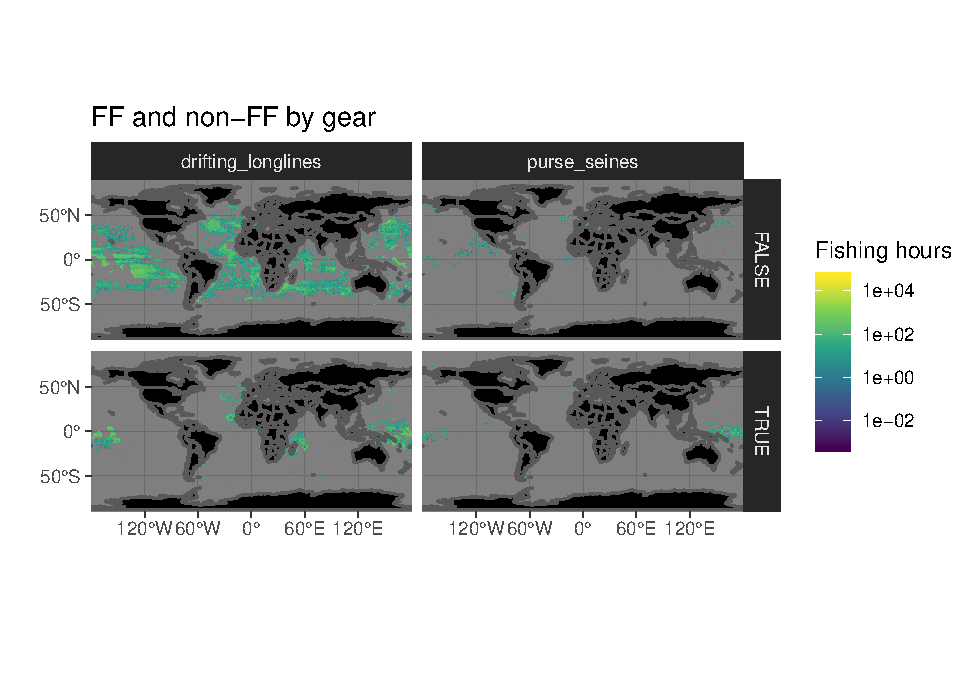
\includegraphics{Oremus_Villasenor-Derbez_files/figure-latex/unnamed-chunk-3-1.pdf}

\subsection{ENSO data}\label{enso-data}

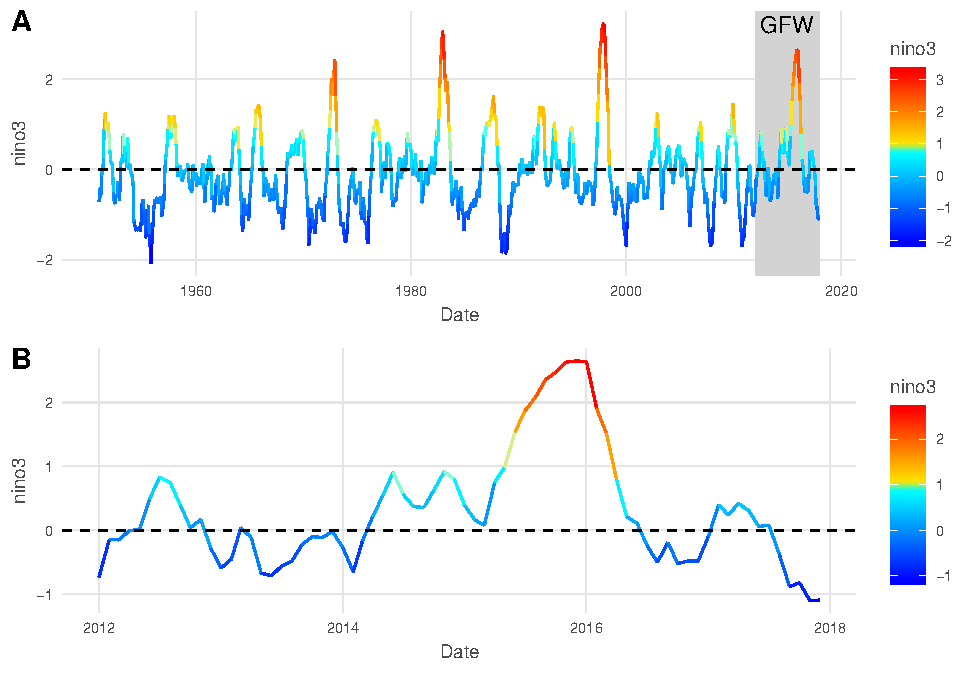
\includegraphics{Oremus_Villasenor-Derbez_files/figure-latex/unnamed-chunk-5-1.pdf}

\subsection{Empirical specifications}\label{empirical-specifications}

\subsubsection{ENSO and Foreign Fishing}\label{enso-and-foreign-fishing}

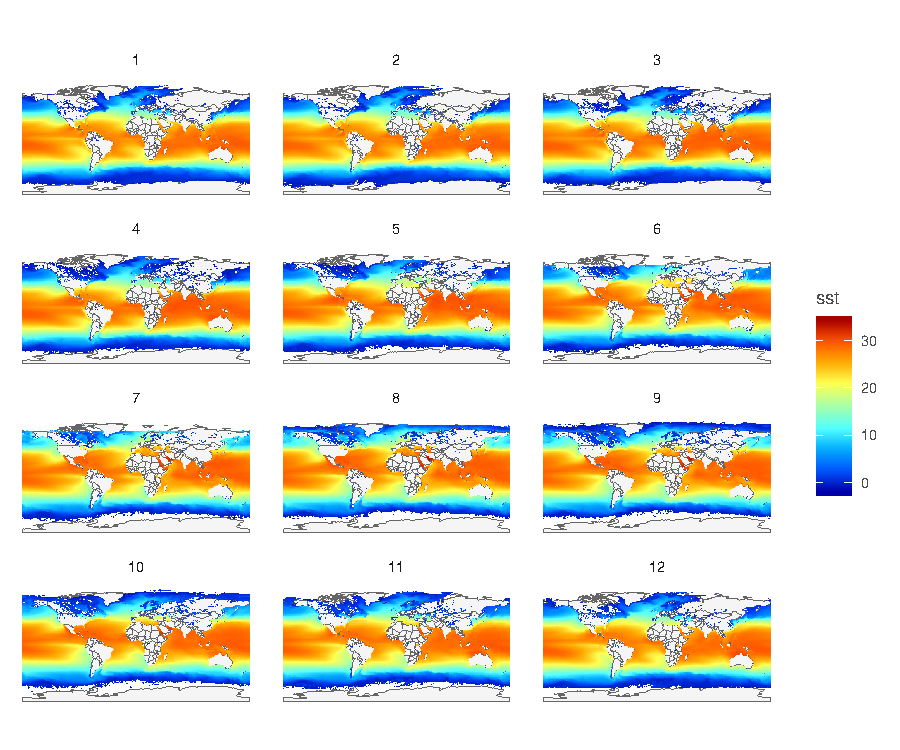
\includegraphics{Oremus_Villasenor-Derbez_files/figure-latex/unnamed-chunk-6-1.pdf}

We estimate the effects of ENSO on Foreign Fishing using a
difference-in-difference strategy to compare the effects of ENSO on
foreign fishing in regions impacted by ENSO to its effects on foreign
fishing in regions not impacted by ENSO.

\[log(FF_{ct}) = \alpha + \beta ENSO_t \times \Pi_{c\epsilon T} + \phi_t + \lambda_c + \epsilon_{ct}\]

\(FF_{ct}\) represents the foreign fishing variable of interest by
country and year. We use an inverse hyperbolic sine\footnote{\(ln(FF + \sqrt{1 + FF^2} \rightarrow ln(2L)\)}
of our foreign fishing variable in my main specification to transform
zeroes in the data \citep{burbidge_1988,card_2017}. \(\alpha\) is a
constant and \(\beta\) captures the linear effect of ENSO on countries
in effected regions compared to counties in regions uneffected by ENSO.
The treatment is ENSO interacted with a dummy, \(\Pi_{ct}\), that equals
1 for countries in ENSO-effected regions and 0 for countries in
uneffected-ENSO regions. \(\phi_t\) are monthly fixed effects and
\(\lambda_c\) are country fixed effects. Standard errors are clustered
at the country level

\subsubsection{Identify treatment
regions}\label{identify-treatment-regions}

First we established a relationship between ENSO and two local
environmental variables that drive the geographical presence of fish
stocks, sea-surface temperature (SST) and windspeed. We use composite
images of average monthly SST value, \(SST_t\) , from the NASA
Dataset\footnote{\url{ftp://podaac-ftp.jpl.nasa.gov/}}. We run the
following regression model:

\[SST_t = \omega + \phi ENSO_t + \sum_{p = 1}^{N}{\mu_pt^p} + \epsilon_t\]

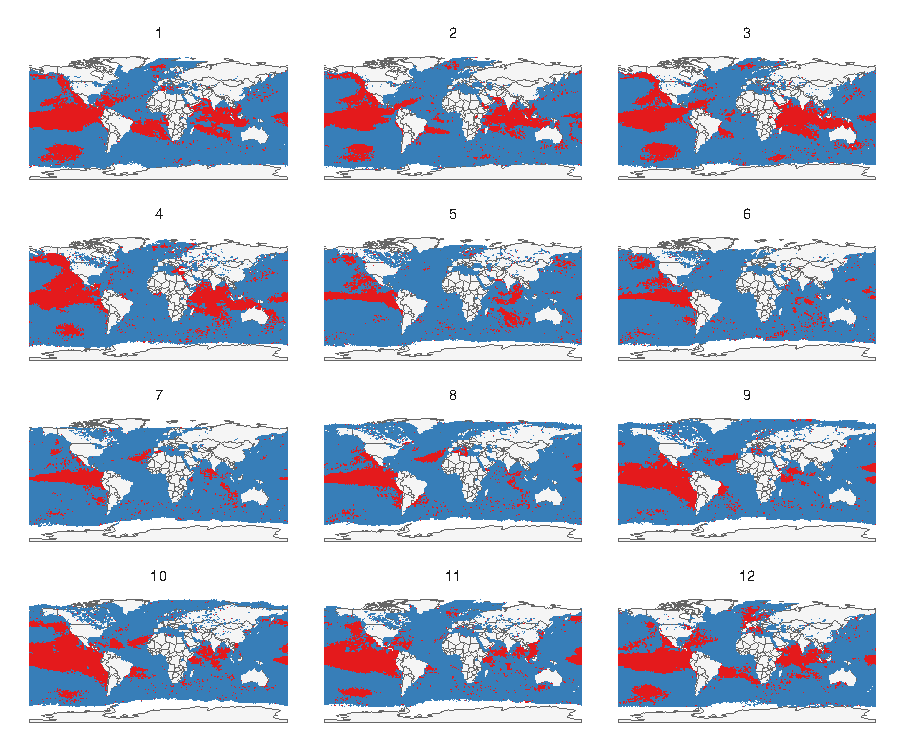
\includegraphics{Oremus_Villasenor-Derbez_files/figure-latex/unnamed-chunk-8-1.pdf}

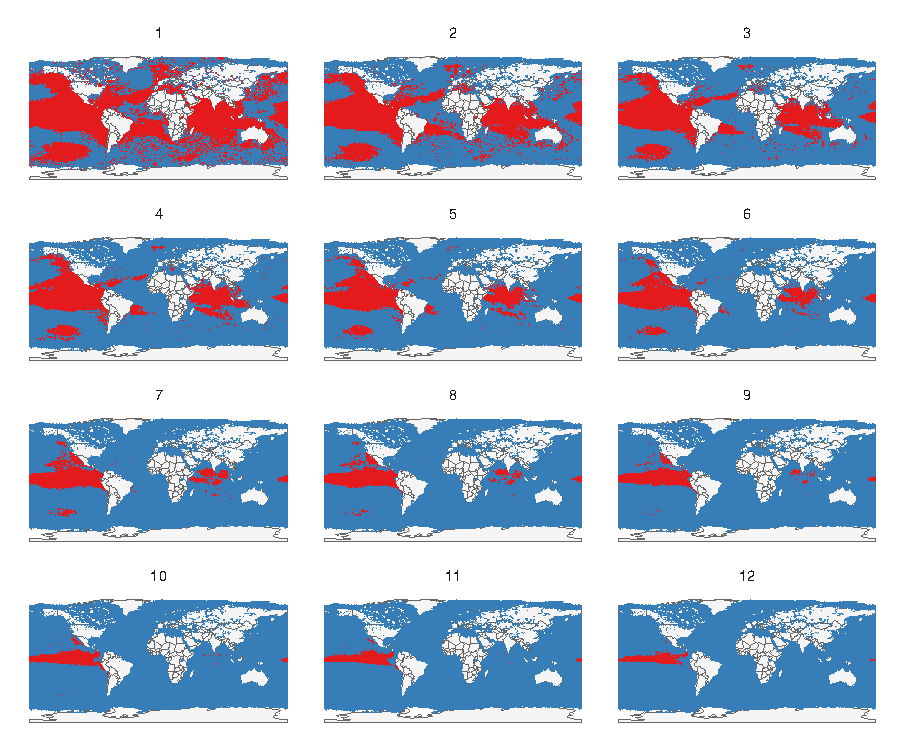
\includegraphics{Oremus_Villasenor-Derbez_files/figure-latex/unnamed-chunk-9-1.pdf}

where \(\omega\) is a constant, \(\phi\) captures the linear effect of
monthly ENSO and µp captures the effect of a p\textsuperscript{th}-order
polynomial time trend. Standard errors use the Newey-West adjustment
which allows for serial correlation and heteroscedasticity of arbitrary
form in the error terms over an optimally chosen window of time
\citep{newey_1987,newey_1994}.

SST during this sample period exhibited trending behavior and thus
needed to be detrended. To determine the polynomial order of the time
trend, \(N\), we use the Akaike Information Criteria (AIC)
\citep{akaike_1974}, which when minimized captures a model's overall
goodness of fit while penalizing additional terms with limited
explanatory power. For both fisheries, we observe that the AIC statistic
drops when a time trend of second-order or higher is included in
Equation 2. Importantly, we detect a positive/negative relationship
between winter ENSO and SST and a positive/negative relationship between
winter ENSO and windspeed, shown in Figure X.

\[log(FF_t) = \psi + \delta ENSO_t + \sum_{p = 1}^{N}{k_pt^p} + \mu_t\]

\(\psi\) is a constant; \(\delta\) captures the linear effect of ENSO
and \(k_p\) represents the effect of a p\textsuperscript{th}-order
polynomial time trend. Standard errors use the Newey-West adjustment,
allowing for arbitrary forms of serial correlation and
heteroscedasticity in the error term with a bandwidth of 10 months. As a
robustness check, we use different polynomial time trends to remove any
long-term trends

\begin{table}[!htbp] \centering 
  \caption{\label{tab:kir_vessels}Foreign fishing hours and nino3} 
  \label{} 
\begin{tabular}{@{\extracolsep{5pt}}lcccc} 
\\[-1.8ex]\hline 
\hline \\[-1.8ex] 
 & \multicolumn{4}{c}{\textit{Dependent variable:}} \\ 
\cline{2-5} 
\\[-1.8ex] & \multicolumn{4}{c}{hours} \\ 
\\[-1.8ex] & (1) & (2) & (3) & (4)\\ 
\hline \\[-1.8ex] 
 nino3anom & 0.718$^{***}$ & 0.748$^{***}$ & 0.753$^{***}$ & 0.438$^{***}$ \\ 
  & (0.075) & (0.076) & (0.076) & (0.077) \\ 
  & & & & \\ 
 treated & $-$0.087 & 0.040 & 0.046 & $-$1.097$^{***}$ \\ 
  & (0.113) & (0.107) & (0.107) & (0.116) \\ 
  & & & & \\ 
 nino3anom:treated & 0.333$^{***}$ & 0.216$^{**}$ & 0.212$^{**}$ & 0.661$^{***}$ \\ 
  & (0.092) & (0.093) & (0.093) & (0.095) \\ 
  & & & & \\ 
 Constant & 19.894$^{***}$ & 19.502$^{***}$ & 19.126$^{***}$ & 19.730$^{***}$ \\ 
  & (0.097) & (0.082) & (0.133) & (1.016) \\ 
  & & & & \\ 
\hline \\[-1.8ex] 
Gear FE & No & Yes & Yes & Yes \\ 
Month FE & No & No & Yes & Yes \\ 
Country FE & No & No & No & Yes \\ 
Observations & 418,458 & 418,458 & 418,458 & 418,458 \\ 
R$^{2}$ & 0.001 & 0.002 & 0.002 & 0.018 \\ 
\hline 
\hline \\[-1.8ex] 
\textit{Note:}  & \multicolumn{4}{r}{$^{*}$p$<$0.1; $^{**}$p$<$0.05; $^{***}$p$<$0.01} \\ 
\end{tabular} 
\end{table}

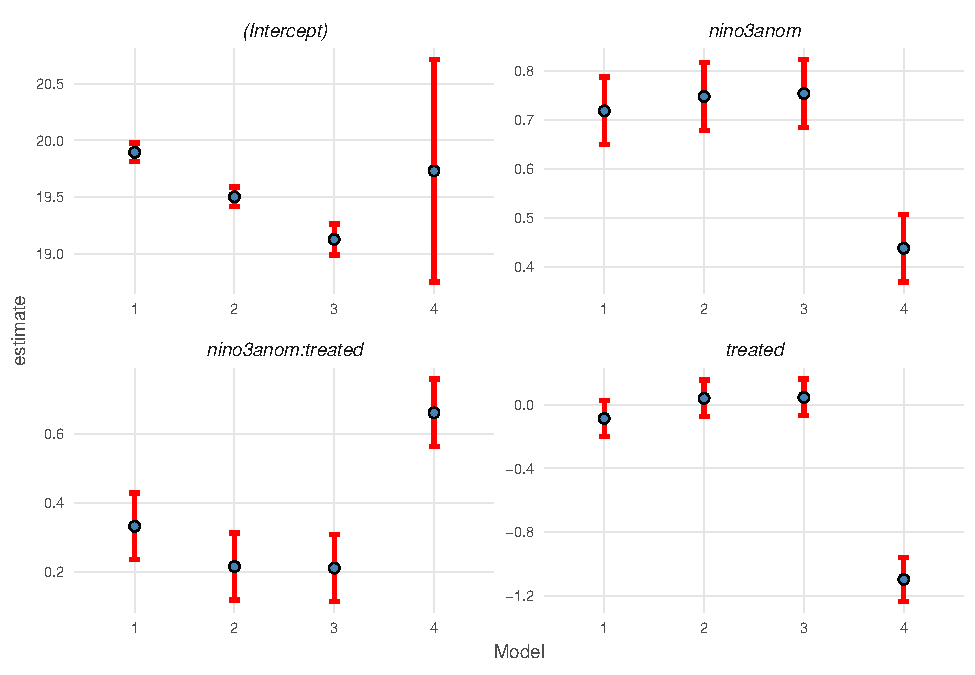
\includegraphics{Oremus_Villasenor-Derbez_files/figure-latex/unnamed-chunk-12-1.pdf}

\clearpage

\renewcommand\refname{References}
\bibliography{references.bib}


\end{document}
